\PassOptionsToPackage{unicode=true}{hyperref} % options for packages loaded elsewhere
\PassOptionsToPackage{hyphens}{url}
\documentclass[11pt,dvipsnames,ignorenonframetext,aspectratio=169]{beamer}
\IfFileExists{pgfpages.sty}{\usepackage{pgfpages}}{}
\setbeamertemplate{caption}[numbered]
\setbeamertemplate{caption label separator}{: }
\setbeamercolor{caption name}{fg=normal text.fg}
\beamertemplatenavigationsymbolsempty
\usepackage{lmodern}
\usepackage{amssymb,amsmath}
\usepackage{ifxetex,ifluatex}
\usepackage{fixltx2e} % provides \textsubscript
\ifnum 0\ifxetex 1\fi\ifluatex 1\fi=0 % if pdftex
  \usepackage[T1]{fontenc}
  \usepackage[utf8]{inputenc}
\else % if luatex or xelatex
  \ifxetex
    \usepackage{mathspec}
  \else
    \usepackage{fontspec}
\fi
\defaultfontfeatures{Ligatures=TeX,Scale=MatchLowercase}







\fi

  \usetheme[]{monash}

  \usecolortheme{monashwhite}


% A default size of 24 is set in beamerthememonash.sty

% Title page
\setbeamertemplate{title page}
{\placefig{-0.01}{-0.01}{width=1.01\paperwidth,height=1.01\paperheight}{drone\_system.jpg}
\begin{textblock}{7.5}(1,2.8)\usebeamerfont{title}
{\color{white}\raggedright\par\inserttitle}
\end{textblock}
\begin{textblock}{7.5}(1,7)
{\color{white}\raggedright{\insertauthor}\mbox{}\\[0.2cm]
\insertdate}
\end{textblock}}


  \useinnertheme{rounded}

  \useoutertheme{smoothtree}

% use upquote if available, for straight quotes in verbatim environments
\IfFileExists{upquote.sty}{\usepackage{upquote}}{}
% use microtype if available
\IfFileExists{microtype.sty}{%
  \usepackage{microtype}
  \UseMicrotypeSet[protrusion]{basicmath} % disable protrusion for tt fonts
}{}


\newif\ifbibliography
  \usepackage[round]{natbib}
  \bibliographystyle{plainnat}


\hypersetup{
      pdftitle={System simulation: Concepts and principles, introduction to CSMs and their uses for agricultural input use optimization},
            colorlinks=true,
    linkcolor=red,
    citecolor=Blue,
    urlcolor=lightgrayd,
    breaklinks=true}
%\urlstyle{same}  % Use monospace font for urls







% Prevent slide breaks in the middle of a paragraph:
\widowpenalties 1 10000
\raggedbottom

  \AtBeginPart{
    \let\insertpartnumber\relax
    \let\partname\relax
    \frame{\partpage}
  }
  \AtBeginSection{
    \ifbibliography
    \else
      \let\insertsectionnumber\relax
      \let\sectionname\relax
      \frame{\sectionpage}
    \fi
  }
  \AtBeginSubsection{
    \let\insertsubsectionnumber\relax
    \let\subsectionname\relax
    \frame{\subsectionpage}
  }



\setlength{\parindent}{0pt}
\setlength{\parskip}{6pt plus 2pt minus 1pt}
\setlength{\emergencystretch}{3em}  % prevent overfull lines
\providecommand{\tightlist}{%
  \setlength{\itemsep}{0pt}\setlength{\parskip}{0pt}}

  \setcounter{secnumdepth}{0}


%% Monash overrides
\AtBeginSection[]{
   \frame<beamer>{
   \frametitle{Outline}\vspace*{0.2cm}
   
   \tableofcontents[currentsection,hideallsubsections]
  }}

% Redefine shaded environment if it exists (to ensure text is black)
\ifcsname Shaded\endcsname
  \definecolor{shadecolor}{RGB}{225,225,225}
  \renewenvironment{Shaded}{\color{black}\begin{snugshade}\color{black}}{\end{snugshade}}
\fi
%%


  \usepackage{setspace}
  \usepackage{wasysym}
  % \usepackage{footnote} % don't use this this breaks all
  \usepackage{fontenc}
  \usepackage{fontawesome}
  \usepackage{booktabs,siunitx}
  \usepackage{longtable}
  \usepackage{array}
  \usepackage{multirow}
  \usepackage{wrapfig}
  \usepackage{float}
  \usepackage{colortbl}
  \usepackage{pdflscape}
  \usepackage{tabu}
  \usepackage{threeparttable}
  \usepackage{threeparttablex}
  \usepackage[normalem]{ulem}
  \usepackage{makecell}
  \usepackage{xcolor}
  \usepackage{tikz} % required for image opacity change
  \usepackage[absolute,overlay]{textpos} % for text formatting
  \usepackage{chemfig}
  \usepackage[skip=0.333\baselineskip]{caption}
  % \newcommand*{\AlignChar}[1]{\makebox[1ex][c]{\ensuremath{\scriptstyle#1}}}%

  % this font option is amenable for beamer
  \setbeamerfont{caption}{size=\tiny}
  \singlespacing
  \definecolor{lightgrayd}{gray}{0.95}
  \definecolor{skyblued}{rgb}{0.65, 0.6, 0.94}
  \definecolor{oranged}{RGB}{245, 145, 200}

  % \newlength{\cslhangindent}
  % \setlength{\cslhangindent}{1.5em}
  % \newenvironment{cslreferences}%
  %   {\setlength{\parindent}{0pt}%
  %   \everypar{\setlength{\hangindent}{\cslhangindent}}\ignorespaces}%
  %   {\par}


  \newcommand{\bcolumns}{\begin{columns}[T, onlytextwidth]}
  \newcommand{\ecolumns}{\end{columns}}

  \newcommand{\bdescription}{\begin{description}}
  \newcommand{\edescription}{\end{description}}

  \newcommand{\bitemize}{\begin{itemize}}
  \newcommand{\eitemize}{\end{itemize}}
  \AtBeginSubsection{}
  \captionsetup{skip=0pt,font=tiny,belowskip=0pt,aboveskip=0pt}
  \usepackage{multicol}

  \title[]{System simulation: Concepts and principles, introduction to
CSMs and their uses for agricultural input use optimization}


  \author[
        Deependra Dhakal\\
Assistant Professor\\
\textit{ddhakal.rookie@gmail.com}\\
\url{https://rookie.rbind.io}
    ]{Deependra Dhakal\\
Assistant Professor\\
\textit{ddhakal.rookie@gmail.com}\\
\url{https://rookie.rbind.io}}


\date[
      
  ]{
    }

\begin{document}

% Hide progress bar and footline on titlepage
  \begin{frame}[plain]
  \titlepage
  \end{frame}


   \frame<beamer>{
   \frametitle{Outline}\vspace*{0.2cm}
   
   \tableofcontents[hideallsubsections]
  }

\hypertarget{system-simulation-concepts-and-principles}{%
\section{System simulation: Concepts and
principles}\label{system-simulation-concepts-and-principles}}

\begin{frame}{}
\protect\hypertarget{section}{}
\bcolumns
\column{0.5\textwidth}


\includegraphics[width=0.9\linewidth]{../images/model_scarlett-johanson-ftr}

\column{0.5\textwidth}

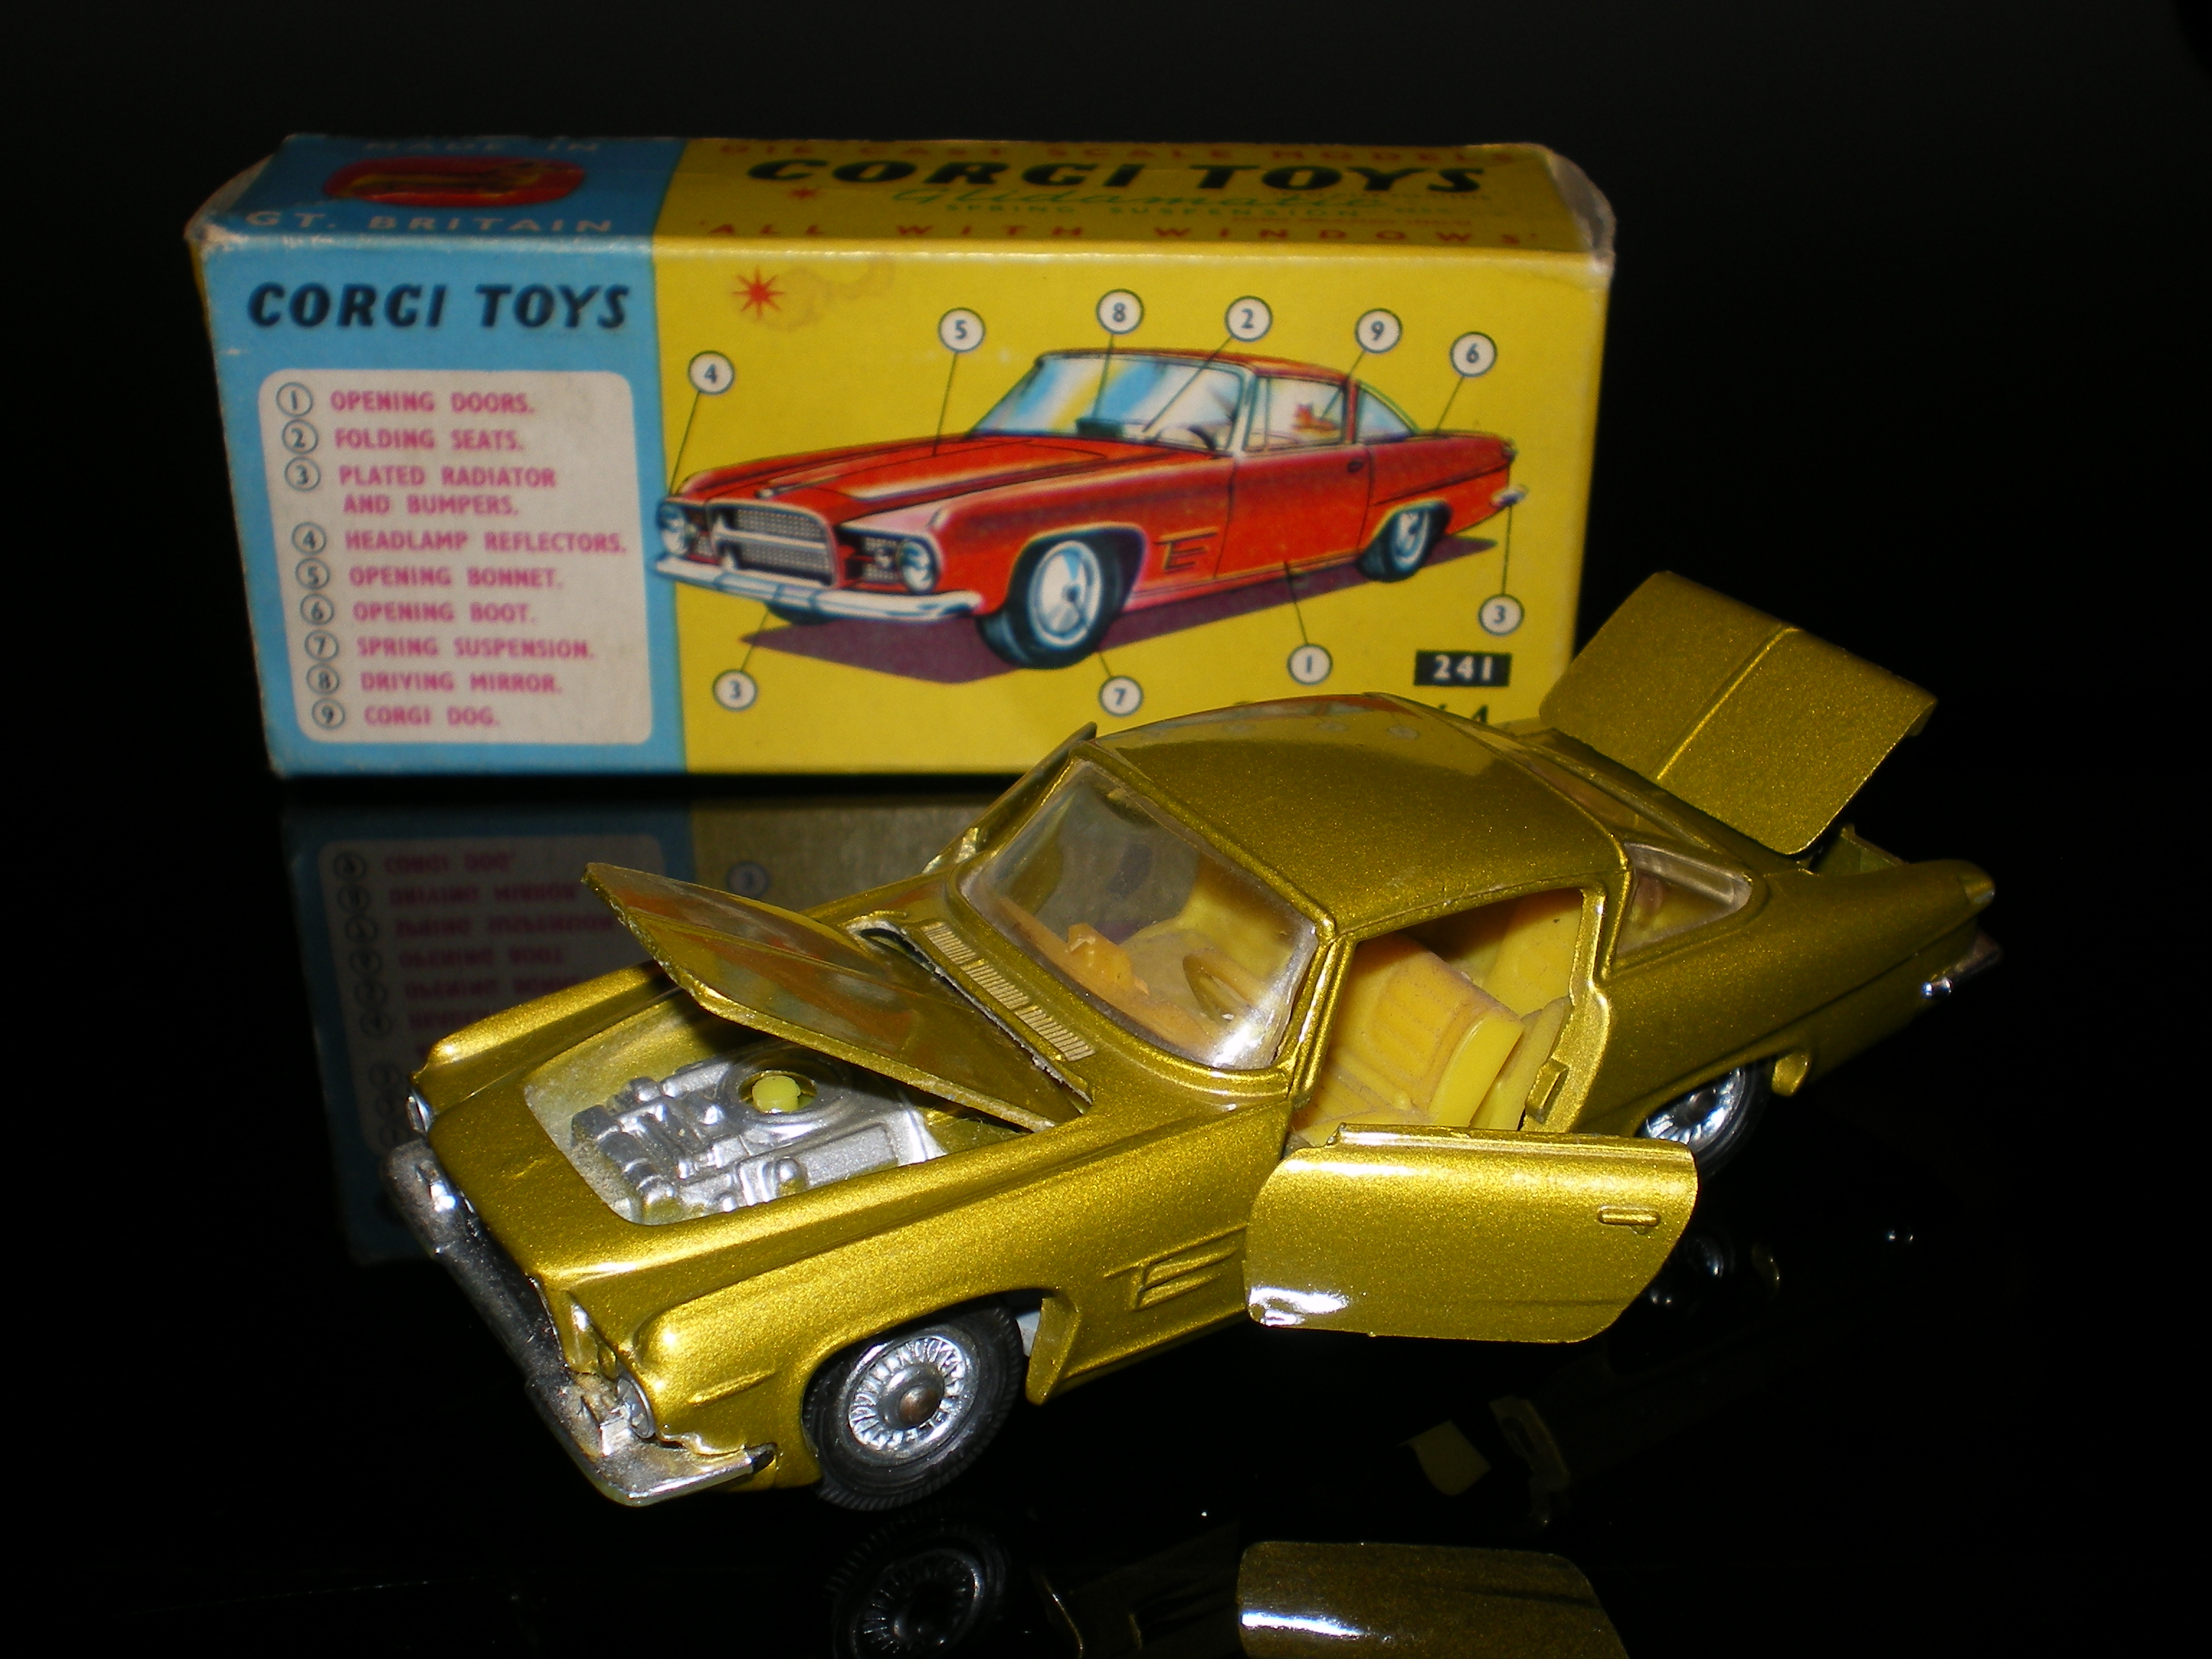
\includegraphics[width=0.8\linewidth]{../images/model_car}

\ecolumns

\centering What's \alert{common} in both ?
\end{frame}

\begin{frame}{Simulation versus model}
\protect\hypertarget{simulation-versus-model}{}
\small

\begin{itemize}
\tightlist
\item
  Simulation is the imitation of the operation of a real-world process
  or system over time.
\item
  Requires the use of models; the model represents the key
  characteristics or behaviors of the selected system or process,
  whereas the simulation represents the evolution of the model over
  time.
\end{itemize}

\begin{figure}
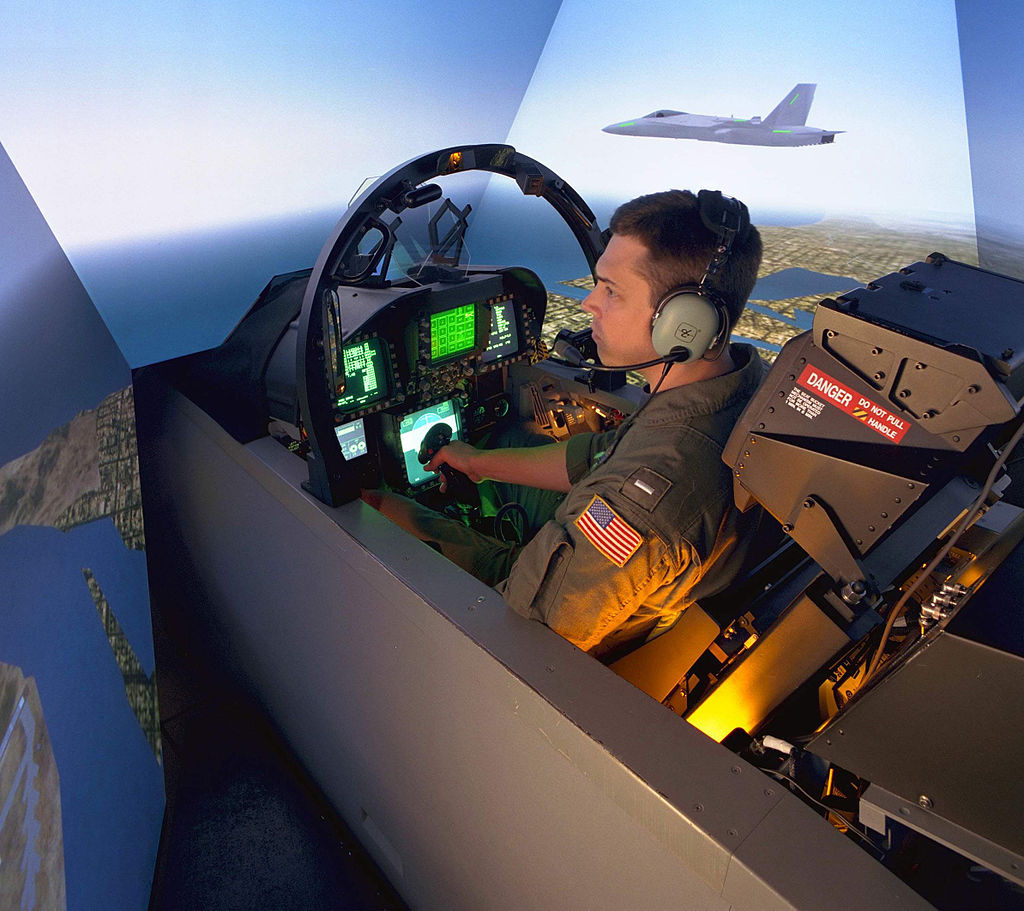
\includegraphics[width=0.55\linewidth]{../images/military_flight_simulator} \caption{A military flight simulator.}\label{fig:flight-simulation}
\end{figure}
\end{frame}

\begin{frame}{}
\protect\hypertarget{section-1}{}
\begin{itemize}
\tightlist
\item
  A thing used as an example to follow or imitate
\item
  A simplified description, especially a mathematical one, of a system
  or process, \(\longrightarrow\) assist calculations and predictions
  \(\longrightarrow\) serve a specific aim.
\item
  \alert{Never} contain all features of reality.
\item
  A system model is a representation of a system, many different
  expression that vary in degree of formalism could be considered
  models.

  \begin{itemize}
  \tightlist
  \item
    A picture
  \item
    A text description
  \end{itemize}
\item
  Primary focus of system modeling is to use models supported by a
  \alert{well-defined} modeling \alert{language}.
\item
  \(\therefore\) \(\uparrow\) the formalism better will be the
  description of the system fitting as a model.
\end{itemize}
\end{frame}

\begin{frame}{Crop (and cropping system) models}
\protect\hypertarget{crop-and-cropping-system-models}{}
\bcolumns
\column{0.7\textwidth}

\begin{itemize}
\tightlist
\item
  Simplification of a crop
\item
  Depending upon the model's goal, several formuations are available.
\item
  Increasing importance:

  \begin{itemize}
  \tightlist
  \item
    Complexity of ecological problems
  \item
    Improved understanding of quantitative relationships in crops
  \item
    Improved computing power
  \end{itemize}
\end{itemize}

\column{0.3\textwidth}

\begin{figure}
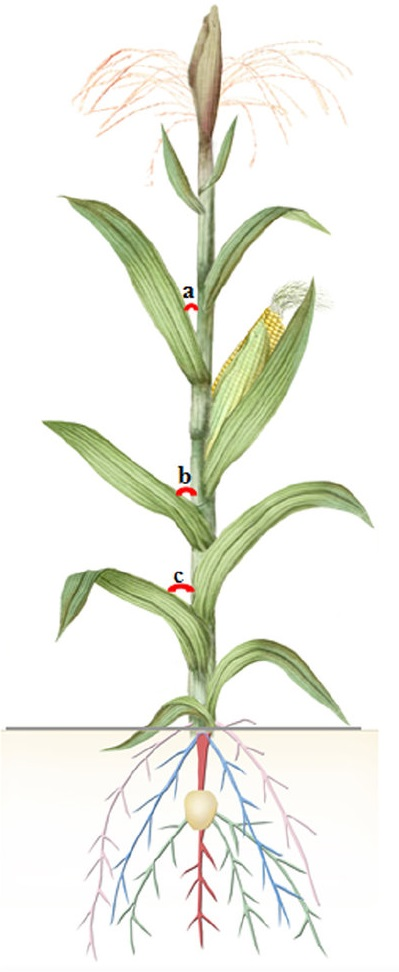
\includegraphics[width=0.36\linewidth]{../images/maize-ideotype} \caption{A diagram of proposed maize ideotype with specific shoot and root traits. Leaf angle (a < b < c) to maximize light capture; Uniform and moderate plant and ear height, etc. to enable mechanized harvest and lodging resistace; Steep, cheap and deep root system to improve water and nutrient uptake. (The roots in shades of different intensities; dark to light represent, respectively, primary roots, seminal roots, crown roots and brace roots.)}\label{fig:crop-model-ideotype}
\end{figure}

\ecolumns
\end{frame}

\begin{frame}{Selected types of models}
\protect\hypertarget{selected-types-of-models}{}
\begin{description}
\small
\item[Static] A model that does not include the time dimension
\item[Dynamic] A model that includes the time dimension
\item[Descriptive/functional] A model that shows the relationshp between the element of a system without any explaination. It is usually unrelated to system structure.
\item[Explanatory/mechanistic] A model that explains the behaviour of a system at an upper integration level by integrating processes of a lower integration level. Representation of the essential system structure.
\item[Deterministic] The predicted values are computed exactly.
\item[Stochastic] The predicted values depend on probability distribution.
\end{description}
\end{frame}

\begin{frame}{}
\protect\hypertarget{section-2}{}
\bcolumns
\column{0.35\textwidth}

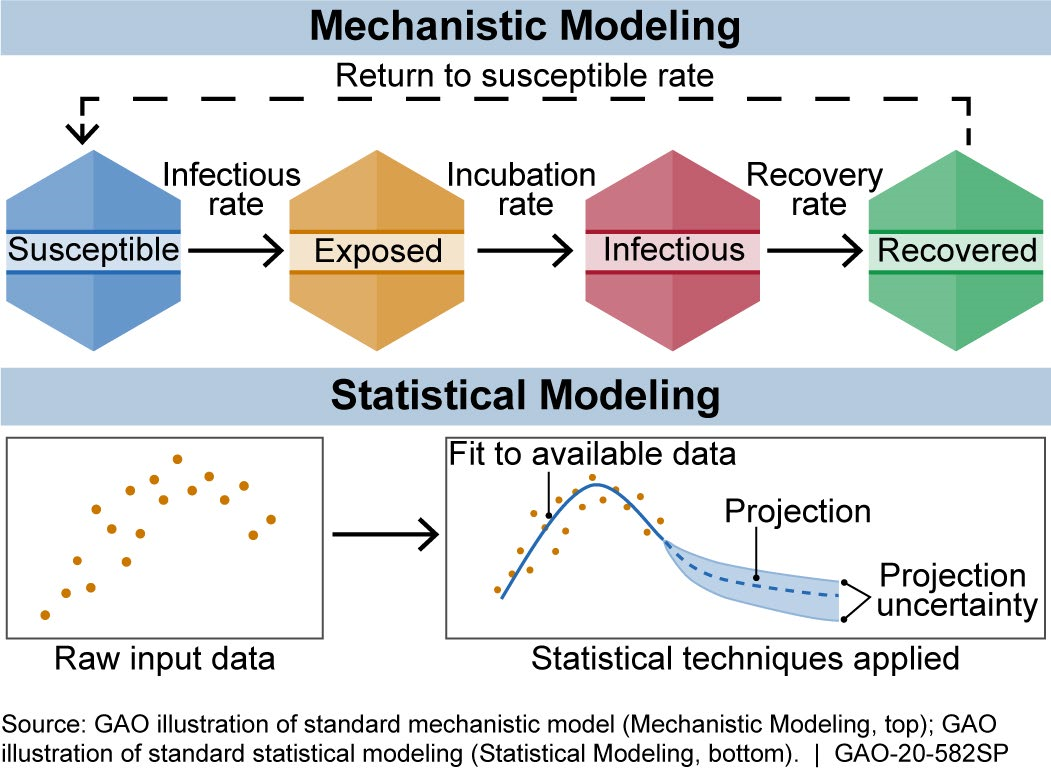
\includegraphics[width=0.95\linewidth]{../images/mechanistic_modeling_COVID_USE}

\column{0.65\textwidth}

\begin{figure}
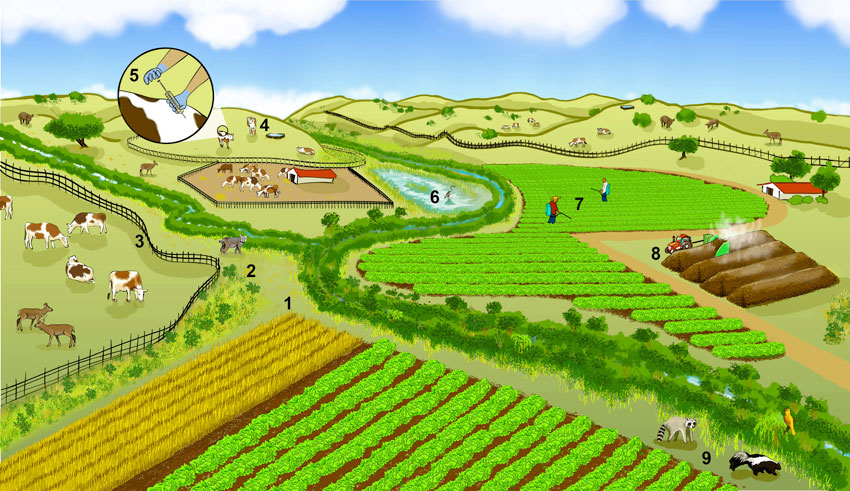
\includegraphics[width=0.92\linewidth]{../images/farminglandscape-numbered-850} \caption{A farming landscape. A representation of processes that make up in farming.}\label{fig:farming-landscape}
\end{figure}

\ecolumns
\end{frame}

\begin{frame}{A model of wheat crop}
\protect\hypertarget{a-model-of-wheat-crop}{}
\begin{figure}
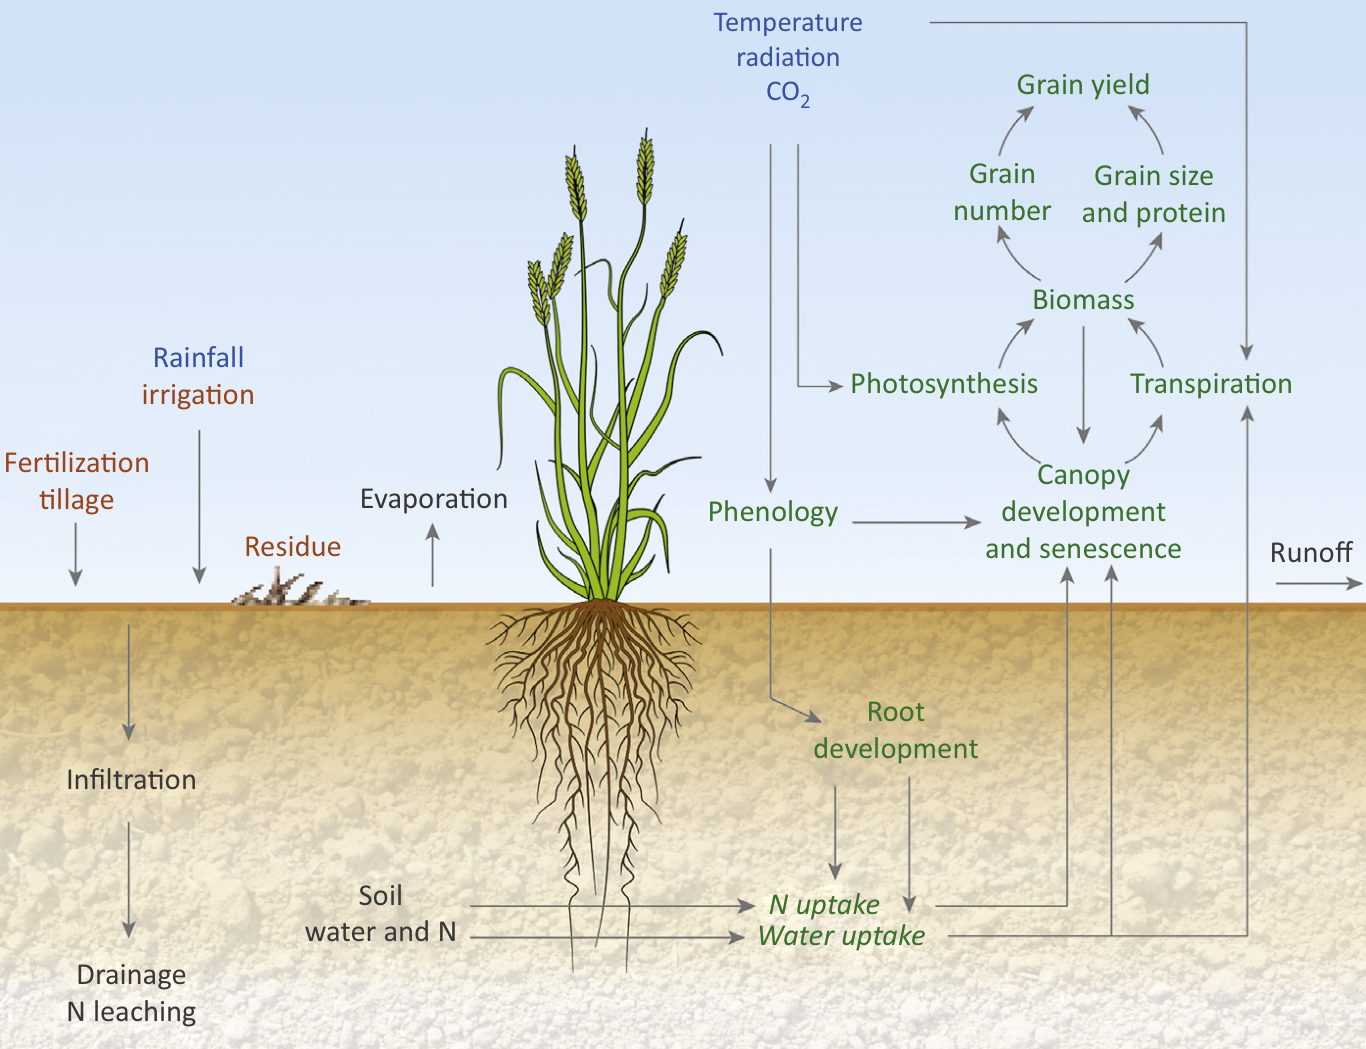
\includegraphics[width=0.42\linewidth]{../images/wheat_mechanistic_processes} \caption{Corp models simulate crop growth and development (outputs) as influenced by climate conditions (typically solar radiation, temperature, and rainfall), soil characteristics (e.g., rooting depth, water holding capacity, nitrogen mineralization capacity) and crop management (e.g., sowing date, plant density, fertilization, irrigation) (inputs) based on mathematical equations and cultivar-specific parameters (inputs). While modern wheat crop models vary in their complexity, most simulate crop growth and development at a daily time-step to ultimately estimate grain yield. Crop processes include phenology driven by temperature and photoperiod, the establishment of the canopy that transpires water and intercepts light to produce the crop biomass, and the partitioning of this biomass into differnt organs including grains. Modeling of soil water and nutrient varies between models, and ranges from simple approaches with no soil description to more complex approaches where soil layers are each described with specific properties. Source: \cite{chenu2017contribution}.}\label{fig:wheat-crop-model}
\end{figure}
\end{frame}

\begin{frame}{Components of crop models}
\protect\hypertarget{components-of-crop-models}{}
\begin{itemize}
\tightlist
\item
  First examples of crop growth models, mostly intended for use by the
  agriculture research community, were available during the 1970s.

  \begin{itemize}
  \tightlist
  \item
    applications oriented to management or field decisions (irrigation
    scheduling, pest and disease control, etc.)
  \end{itemize}
\item
  Now several modeling systems simulate,

  \begin{multicols}{3}
  \begin{itemize}
  \footnotesize
  \item soil water budget,
  \item soil-plant nitrogen budget,
  \item crop phenology,
  \item canopy and root growth,
  \item biomass production,
  \item crop yield,
  \item residue production and decomposition,
  \item soil erosion by water,
  \item and salinity
  \end{itemize}
  \end{multicols}
\item
  These processes are affected by weather, soil characteristics, crop
  characteristics, and cropping system management options including crop
  rotation, cultivar selection, irrigation, nitrogen fertilization, soil
  and irrigation, water salinity, tillage operations, and residue
  management.
\end{itemize}
\end{frame}

\begin{frame}{Process based modeling}
\protect\hypertarget{process-based-modeling}{}
\begin{itemize}
\tightlist
\item
  Crop models need to be \alert{complete} and \alert{responsive}.
\item
  Process based models are easy to describe, most flexible (in terms of
  component addition and substitution).

  \begin{itemize}
  \tightlist
  \item
    Biomass accumulation based models are not always sufficient as
    changes depend on earlier effects (fallow period, previous crop,
    etc.)
  \end{itemize}
\end{itemize}

\begin{figure}
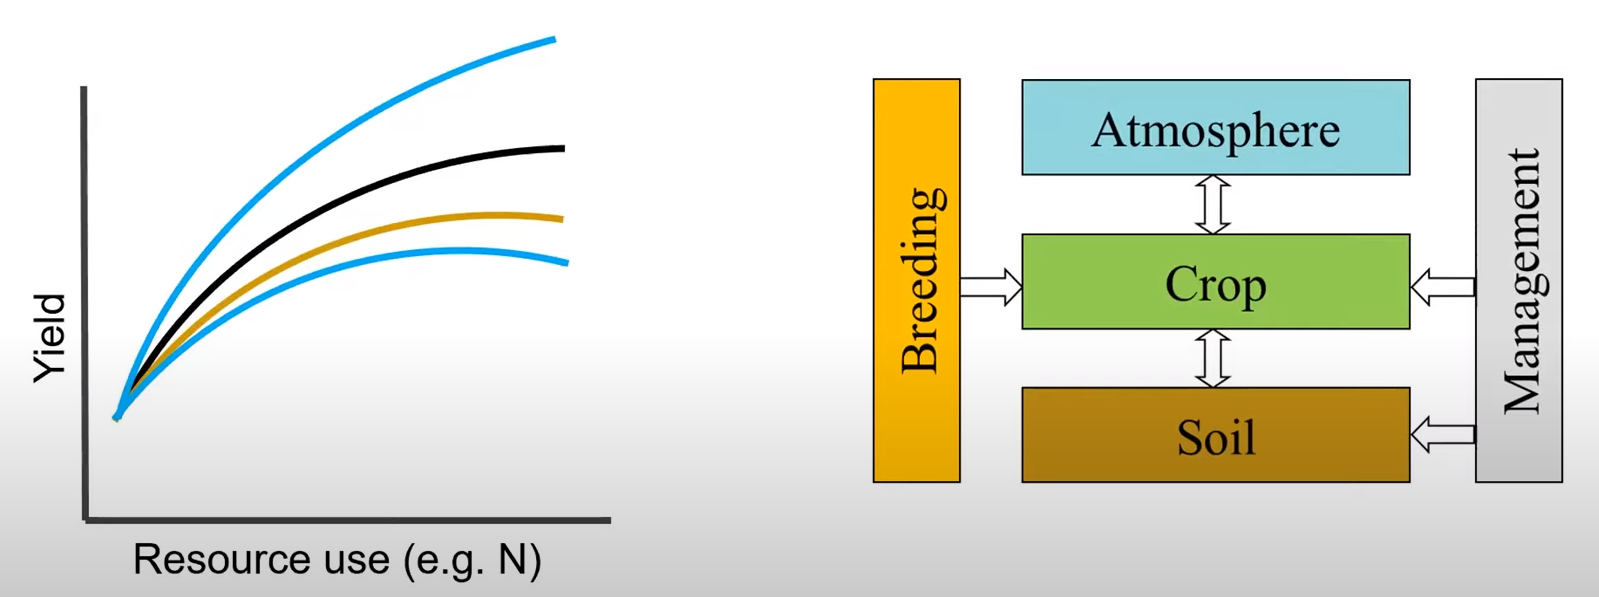
\includegraphics[width=0.75\linewidth]{../images/complex_interaction_factors} \caption{Resonse of yield to mangement can be simulated by an example response to crop yield yield by doses of Nitrogen. Quality of the interaction is generally same but the quantitative nature of interaction is complex.}\label{fig:process-based-models}
\end{figure}
\end{frame}

\hypertarget{example-of-crop-models}{%
\section{Example of crop models}\label{example-of-crop-models}}

\begin{frame}{Biomass accumulation model}
\protect\hypertarget{biomass-accumulation-model}{}
\bcolumns
\column{0.35\textwidth}
\begin{figure}
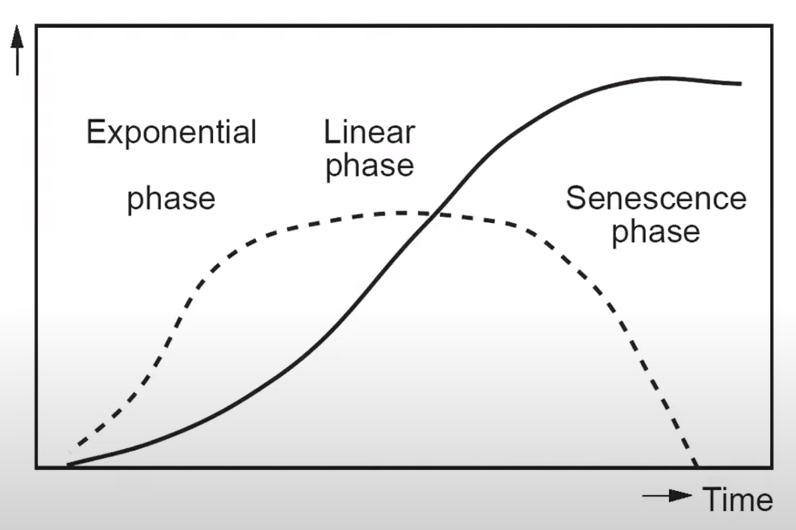
\includegraphics[width=0.9\linewidth]{../images/crop_growth_model_phenology_based} \caption{Simplified model of crop growth based on phenology.}\label{fig:crop-growth-model-simple}
\end{figure}

\column{0.65\textwidth}

\begin{figure}
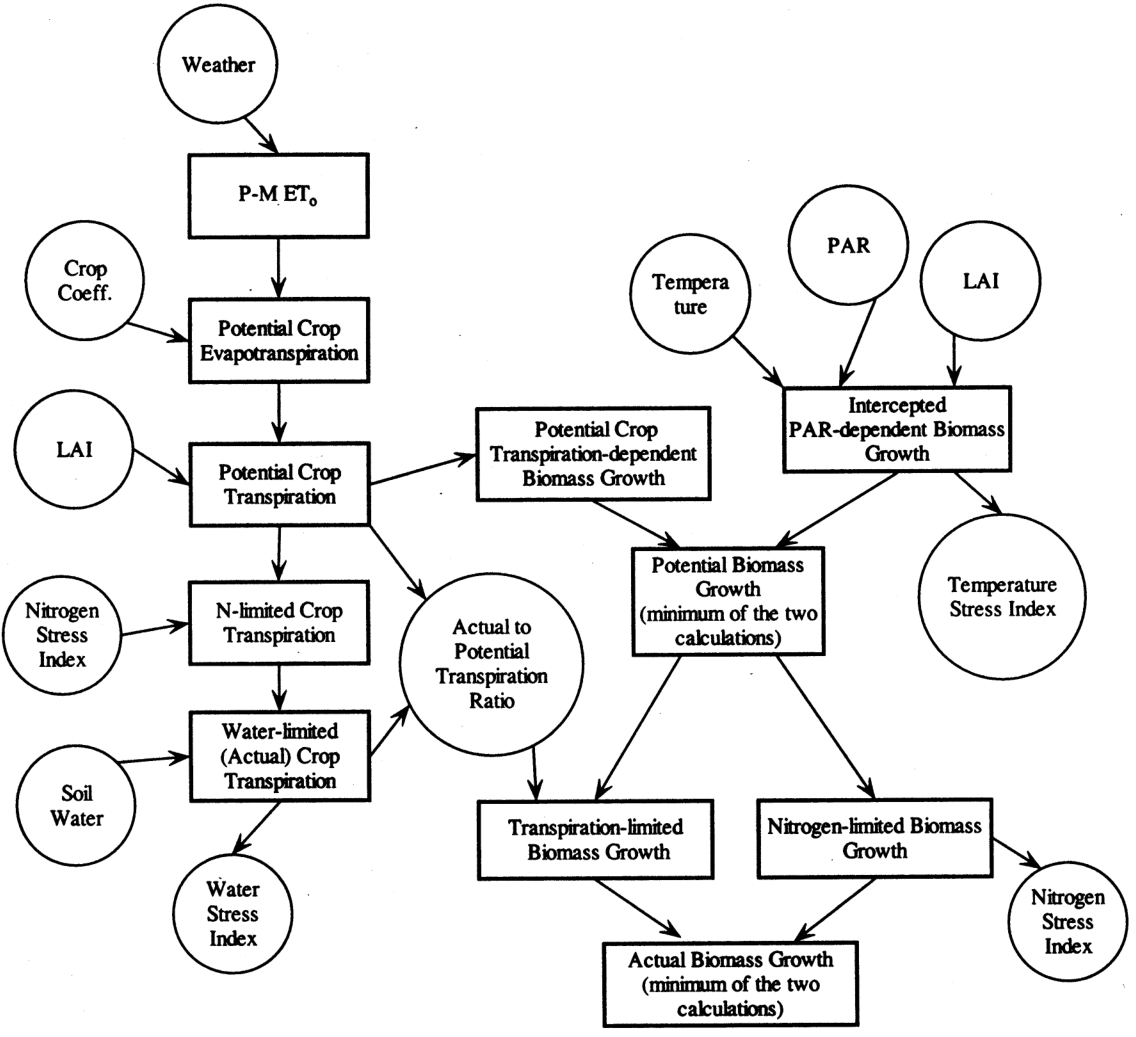
\includegraphics[width=0.72\linewidth]{../images/biomass_growth_model} \caption{Flowchart of biomass growth calculations (in CropSyst). Source: \cite{stockle2003cropsyst}.}\label{fig:biomass-growth-model}
\end{figure}

\ecolumns
\end{frame}

\begin{frame}{}
\protect\hypertarget{section-3}{}
\begin{figure}
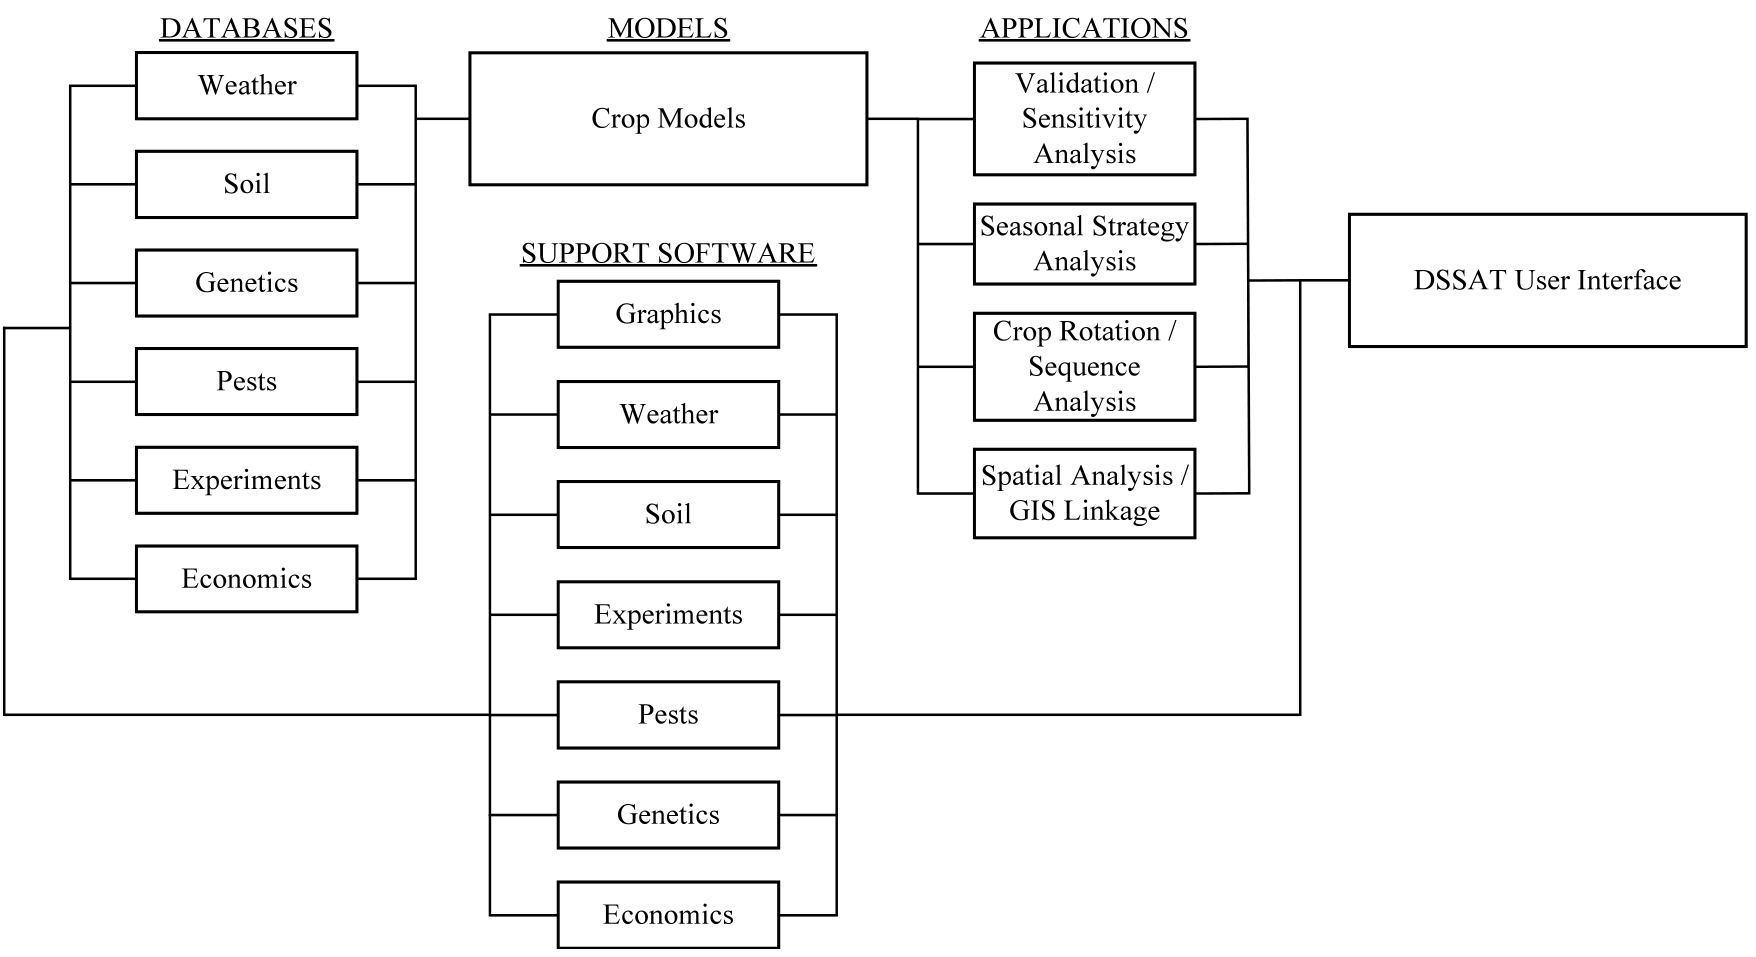
\includegraphics[width=0.8\linewidth]{../images/csm_dssat_framework} \caption{Diagram of database, application, and support software components and their use with crop models for applications in DSSAT.}\label{fig:dssat-framework}
\end{figure}
\end{frame}

\begin{frame}{Steps in crop modeling}
\protect\hypertarget{steps-in-crop-modeling}{}
\bcolumns
\column{0.2\textwidth}
\footnotesize

\begin{itemize}
\tightlist
\item
  Broadly

  \begin{itemize}
  \scriptsize
  \item Model operation
  \item Model evaluation
    \begin{itemize}
    \scriptsize
    \item calibration
    \item validation
    \end{itemize}
  \end{itemize}
\end{itemize}

\column{0.8\textwidth}

\begin{figure}
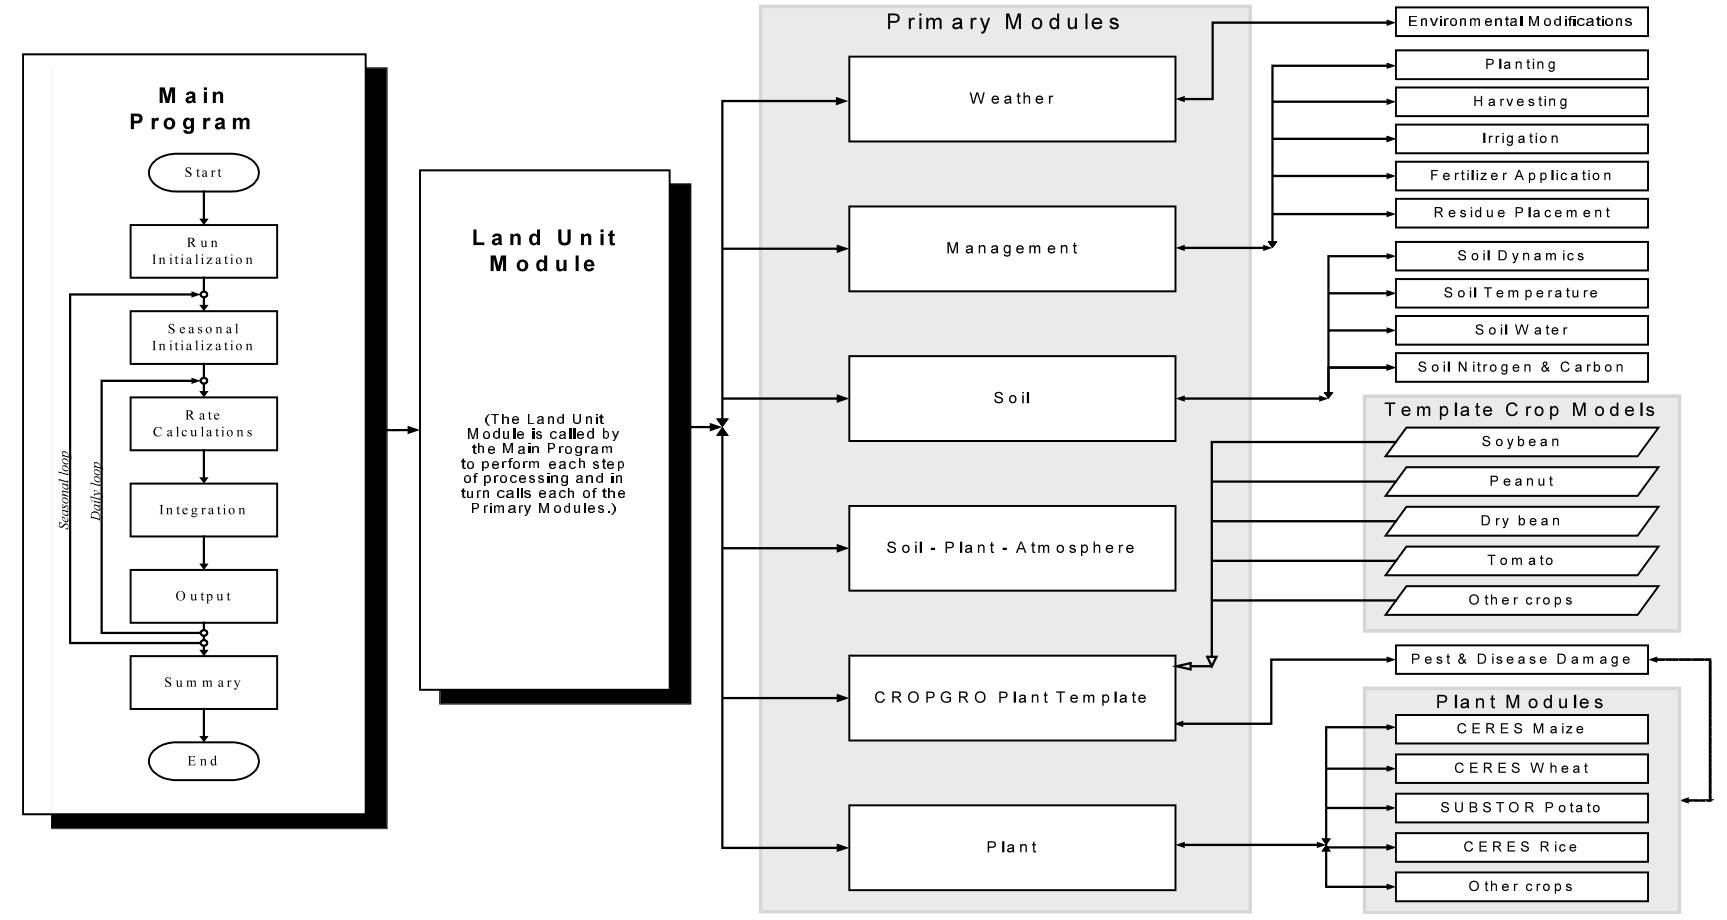
\includegraphics[width=0.88\linewidth]{../images/modular_operation_dssat} \caption{Overview of the components and modular structure of the DSSAT-CSM. Source: \cite{jones2003dssat}.}\label{fig:modular-organization-dssat}
\end{figure}

\ecolumns
\end{frame}

\hypertarget{bibliography}{%
\section{Bibliography}\label{bibliography}}

\begin{frame}{References}
\protect\hypertarget{references}{}
\end{frame}

          \begin{frame}[allowframebreaks]{}
    \bibliographytrue
    \bibliography{./../bibliographies.bib}
    \end{frame}
  


\end{document}
